\documentclass{jhwhw}

\title{Tutorial A7\\Vectors I}
\author{Eytan Chong}
\date{2024-05-02}

\begin{document}
    \problem{}
        The vector $\vec v$ is defined by $3\vec i - 4 \vec j + \vec k$. Find the unit vector in the direction of $\vec v$ and hence find a vector of magnitude 25 which is parallel to $\vec v$.

    \solution
        \begin{align*}
            \vec{\hat v} &= \dfrac{\vec v}{\abs{\vec v}}\\
            &= \dfrac{1}{\sqrt{3^2 + (-4^2) + 1^2}} \cveciii{3}{-4}{1}\\
            &= \dfrac{1}{\sqrt{26}} \cveciii{3}{-4}{1}
        \end{align*}

        \boxt{
            $\dfrac{1}{\sqrt{26}} \cveciii{3}{-4}{1}$, $\dfrac{25}{\sqrt{26}} \cveciii{3}{-4}{1}$
        }

    \problem{}
        With respect to an origin $O$, the position vectors of the points $A$, $B$, $C$ and $D$ are $4\vec i + 7 \vec j$, $\vec i + 3 \vec j$, $2\vec i + 4 \vec j$ and $3\vec i + d\vec j$ respectively.

        \begin{enumerate}
            \item Find the vectors $\overrightarrow{BA}$ and $\overrightarrow{BC}$.
            \item Find the value of $d$ if $B$, $C$ and $D$ are collinear. State the ratio $\dfrac{BC}{BD}$.
        \end{enumerate}

    \solution
        \part
            \begin{equation*}
                \overrightarrow{BA} = \overrightarrow{OA} - \overrightarrow{OB} = \cvecii47 - \cvecii13 = \cvecii34
            \end{equation*}

            \boxt{
                $\overrightarrow{BA} = \cvecii34$
            }
            \begin{equation*}
                \overrightarrow{BC} = \overrightarrow{OC} - \overrightarrow{OB} = \cvecii24 - \cvecii13 = \cvecii11
            \end{equation*}

            \boxt{
                $\overrightarrow{BC} = \cvecii11$
            }
        
        \part
            If $B$, $C$ and $D$ are collinear, then $\overrightarrow{BC} = \lambda \overrightarrow{CD}$ for some $\lambda$.
            \begin{alignat*}{2}
                &&\overrightarrow{BC} &= \lambda \overrightarrow{CD}\\
                \implies&&\cvecii11 &= \lambda\left(\overrightarrow{OD} - \overrightarrow{OC}\right)\\
                && &= \lambda\left(\cvecii3d - \cvecii24\right)\\
                && &= \cvecii{\lambda}{\lambda(d-4)}
            \end{alignat*}

            Hence, $\lambda = 1$ and $\lambda(d - 4) = 1$, whence $d = 5$.

            \boxt{
                $d = 5$
            }
            \begin{align*}
                \dfrac{BC}{BD} = \dfrac{BC}{BC + CD} = \dfrac{BC}{BC + BC} = \dfrac12
            \end{align*}

            \boxt{
                $\dfrac{BC}{BD} = \dfrac12$
            }

    \problem{}
        The diagram shows a roof, with horizontal rectangular base $OBCD$, where $OB = 10$ m and $BC = 6$ m. The triangular planes $ODE$ and $BCF$ are vertical and the ridge $EF$ is horizontal to the base. The planes $OBFE$ and $DCFE$ are each inclined at an angle $\theta$ to the horizontal, where $\tan \theta = \dfrac43$. The point $O$ is taken as the origin and vectors $\vec i$, $\vec j$, $\vec k$, each of length 1 m, are taken along $OB$, $OD$ and vertically upwards from $O$ respectively.

        \begin{center}
            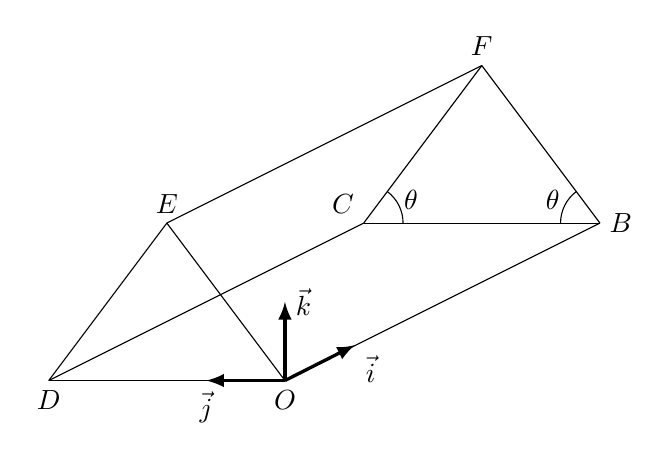
\begin{tikzpicture}
                \draw (0, 0) -- (-3, 0);
                \draw (0, 0) -- (-1.5, 2);
                \draw (-1.5, 2) -- (-3, 0);
                \draw (0, 0) -- (4, 2);
                \draw (4, 2) -- (1, 2);
                \draw (4, 2) -- (2.5, 4);
                \draw (2.5, 4) -- (1, 2);
                \draw (1, 2) -- (-3, 0);
                \draw (2.5, 4) -- (-1.5, 2);

                \node[anchor=north] at (0, 0) {$O$};
                \node[anchor=north] at (-3, 0) {$D$};
                \node[anchor=south] at (-1.5, 2) {$E$};
                \node[anchor=south] at (2.5, 4) {$F$};
                \node[anchor=south east] at (1, 2) {$C$};
                \node[anchor=west] at (4, 2) {$B$};

                \draw (1.5, 2) arc (0:53:0.5);
                \draw (3.5, 2) arc (180:127:0.5);
                \node at (1.6, 2.3) {$\theta$};
                \node at (3.4, 2.3) {$\theta$};

                \draw[very thick, -latex] (0, 0) -- (-1, 0) node[anchor=north] {$\vec j$};
                \draw[very thick, -latex] (0, 0) -- (0, 1) node[anchor=west] {$\vec k$};
                \draw[very thick, -latex] (0, 0) -- (0.89, 0.45) node[anchor=north west] {$\vec i$};
            \end{tikzpicture}
        \end{center}

        \noindent Find the position vectors of the points $B$, $C$, $D$, $E$ and $F$.

    \solution
        Since $OB = 10$ m, we know $\overrightarrow{OB} = 10 \vec i$. Further, since $BC = 6$, we know $\overrightarrow{BC} =  6 \vec j$. Thus, $\overrightarrow{OC} = \overrightarrow{OB} + \overrightarrow{BC} = 10 \vec i + 6 \vec j$.

        Note that $\triangle ODE \cong \triangle BCF$. Hence, $BC \cong OD \implies \overrightarrow{OD} = 6 \vec j$. 
        
        We also have $\angle ODE = \angle DOE = \theta$. Thus, $\triangle ODE$ is isoceles. Let $G$ be the mid-point of $OD$. Since $\tan \theta = \dfrac43$, we have $\dfrac{EG}{DG} = \dfrac43$, which implies that $EG = \dfrac43 DG = \dfrac23 OD$. Thus, $EG = \dfrac23 \cdot 6 = 4$ m. Hence, $\overrightarrow{OE} = \overrightarrow{OG} + \overrightarrow{GE} = \dfrac12 \overrightarrow{OD} + \overrightarrow{GE} = 3\vec j + 4 \vec k$.

        Since $BF \cong OE$, we know $\overrightarrow{BF} = \overrightarrow{OE}$. Thus, $\overrightarrow{OF} = \overrightarrow{OB} + \overrightarrow{BF} = 10 \vec i + 3 \vec j + 4 \vec k$.

        \boxt{
            $
                \begin{aligned}
                    \overrightarrow{OB} &= 10 \vec i\\
                    \overrightarrow{OC} &= 10 \vec i + 6 \vec j\\
                    \overrightarrow{OD} &= 6 \vec j\\
                    \overrightarrow{OE} &= 3 \vec j + 4 \vec k\\
                    \overrightarrow{OF} &= 10 \vec i + 3 \vec j + 4 \vec k
                \end{aligned}
            $
        }

    \problem{}
        Find $\vec u \cdot \vec v$, $\vec u \times \vec v$ and the angle between $\vec u$ and $\vec v$ given that

        \begin{enumerate}
            \item $\vec u = \vec i - \vec j + \vec k$, $\vec v = 3\vec i + 2 \vec j + 7 \vec k$
            \item $\vec u = 2\vec i - 3\vec k$, $\vec v = -\vec i + 7 \vec j + 2\vec k$
        \end{enumerate}

    \solution
        \part
            We have $\vec u = \cveciii1{-1}1$ and $\vec v = \cveciii327$. Hence,
            \begin{align*}
                \vec u \cdot \vec v &= 1 \cdot 3 + (-1) \cdot 2 + 1 \cdot 7\\
                &= 8\\
                \vec u \times \vec v &= \cveciii{-1\cdot7-2\cdot1}{1\cdot3-7\cdot1}{1\cdot2-3\cdot(-1)}\\
                &= \cveciii{-9}{-4}{5}
            \end{align*}

            Let the angle between $\vec u$ and $\vec v$ be $\theta$.
            \begin{alignat*}{2}
                &&\vec u \cdot \vec v &= \abs{\vec u} \abs{\vec v} \cos \theta\\
                \implies&&8 &= \sqrt{1^2 + (-1)^2 + 1^2} \cdot \sqrt{3^2 + 2^2 + 7^2} \cdot \cos \theta\\
                \implies&&\theta &= \arccos \left(\dfrac{8}{\sqrt 3 \cdot \sqrt{62}}\right)\\
                && &= 54.1^\circ \todp{1}
            \end{alignat*}

            \boxt{
                $
                    \begin{aligned}
                        \vec u \cdot \vec v &= 8\\
                        \vec u \times \vec v &= -9 \vec i -4 \vec j + 5 \vec k\\
                        \theta &= 54.1^\circ
                    \end{aligned}
                $
            }

        \part
            We have $\vec u = \cveciii20{-3}$ and $\vec v = \cveciii{-1}72$. Hence,
            \begin{align*}
                \vec u \cdot \vec v &= 2\cdot(-1) + 0 \cdot7 + (-3)\cdot2\\
                &= -8\\
                \vec u \times \vec v &= \cveciii{0\cdot2-7\cdot(-3)}{(-3)\cdot(-1)-2\cdot2}{2\cdot7-(-1)\cdot0}\\
                &= \cveciii{21}{-1}{14}
            \end{align*}

            Let the angle between $\vec u$ and $\vec v$ be $\theta$.
            \begin{alignat*}{2}
                &&\vec u \cdot \vec v &= \abs{\vec u} \abs{\vec v} \cos \theta\\
                \implies&&8 &= \sqrt{2^2 + 0^2 + (-3)^2} \cdot \sqrt{(-1)^2 + 7^2 + 2^2} \cdot \cos \theta\\
                \implies&&\theta &= \arccos \left(\dfrac{-8}{\sqrt{13} \cdot \sqrt{54}}\right)\\
                && &= 107.6^\circ \todp{1}
            \end{alignat*}

            \boxt{
                $
                    \begin{aligned}
                        \vec u \cdot \vec v &= -8\\
                        \vec u \times \vec v &= 21 \vec i - \vec j + 14 \vec k\\
                        \theta &= 107.6^\circ
                    \end{aligned}
                $
            }

    \problem{}
        Find $\vec u \cdot \vec v$ and $\abs{\vec u \times \vec v}$ given that $\vec u = 2\vec a - \vec b$, $\vec v = -\vec a + 3 \vec b$, where $\abs{\vec a} = 2$, $\abs{\vec b} = 1$ and the angle between $\vec a$ and $\vec b$ is 60$^\circ$.

    \solution
        \begin{align*}
            \vec u \cdot \vec v &= (2 \vec a - \vec b) \cdot (-\vec a + 3 \vec b)\\
            &= -2\vec a \cdot \vec a + 6 \vec a \cdot \vec b + \vec b \cdot \vec a -3 \vec b \cdot \vec b\\
            &= -2 \abs{\vec a}^2 - 3 \abs{\vec b}^2 + 7 \abs{\vec a}\abs{\vec b}\cos \theta\\
            &= -2 \cdot 2^2 - 3 \cdot 1^2 + 7 \cdot 2 \cdot 1 \cdot \cos 60^\circ\\
            &= -4\\
            \abs{\vec u \times \vec v} &= \abs{(2 \vec a - \vec b) \times (-\vec a + 3 \vec b)}\\
            &= \abs{-2\vec a \times \vec a + 6 \vec a \times \vec b + \vec b \times \vec a -3 \vec b \times \vec b}\\
            &= \abs{-2 \cdot 0 + 6 \vec a \times \vec b - \vec a \times \vec b -3 \cdot 0}\\
            &= \abs{5 \vec a \times \vec b}\\
            &= 5 \abs{\vec a} \abs{\vec b} \sin \theta\\
            &= 5 \cdot 2 \cdot 1 \cdot \dfrac{\sqrt3}2\\
            &= 5\sqrt3
        \end{align*}

        \boxt{
            $
                \begin{aligned}
                    \vec u \cdot \vec v &= -4\\
                    \abs{\vec u \times \vec v} &= 5 \sqrt3
                \end{aligned}
            $
        }

    \problem{}
        If $\vec a = \vec i + 4 \vec j - \vec k$, $\vec b = \vec i - \vec j + 3 \vec k$ and $\vec c = 2 \vec i + \vec j$, find

        \begin{enumerate}
            \item a unit vector perpendicular to both $\vec a$ and $\vec b$,
            \item a vector perpendicular to both $(3 \vec b - 5 \vec c)$ and $(7 \vec b + \vec c)$.
        \end{enumerate}

    \solution
        \part
            \begin{alignat*}{2}
                &&\vec a \times \vec b &= \cveciii{4\cdot3-(-1)\cdot(-1)}{(-1)\cdot1 - 3\cdot1}{1\cdot(-1)-1\cdot4}\\
                && &= \cveciii{11}{-4}{-5}\\
                \implies&&\abs{\vec a \times \vec b} &= \sqrt{11^2 + (-4)^2 + (-5)^2}\\
                && &= \sqrt{162}\\
                \implies&&\widehat{\vec a \times \vec b} &= \dfrac{1}{\sqrt{162}} \cveciii{11}{-4}{-5}
            \end{alignat*}

            \boxt{
                $\dfrac{1}{\sqrt{162}} \cveciii{11}{-4}{-5}$
            }

        \part
            Observe that $(3 \vec b - 5 \vec c) \times (7 \vec b + \vec c) = \lambda \vec b \times \vec c$ for some scalar $\lambda$. It hence suffices to find $\vec b \times \vec c$.

            \begin{align*}
                \vec b \times \vec c &= \cveciii{(-1)\cdot0 - 1 \cdot3}{3\cdot2 - 0\cdot1}{1 \cdot1-2\cdot(-1)}\\
                &= \cveciii{-3}63
            \end{align*}

            \boxt{
                $\cveciii{-3}63$
            }

    \problem{}
        The position vectors of the points $A$, $B$ and $C$ are given by $\vec a = 2 \vec i + 3 \vec j - 4 \vec k$, $\vec b = 5 \vec i - \vec j + 2 \vec k$, $\vec c = 11 \vec i + \lambda \vec j + 14 \vec k$ respectively. Find

        \begin{enumerate}
            \item a unit vector parallel to $\overrightarrow{AB}$;
            \item the position vector of the point $D$ such that $ABCD$ is a parallelogram, leaving your answer in terms of $\lambda$;
            \item the value of $\lambda$ if $A$, $B$ and $C$ are collinear;
            \item the position vector of the point $P$ on $AB$ is $AP:PB = 2:1$.
        \end{enumerate}

    \solution
        \part
            \begin{align*}
                \overrightarrow{AB} &= \vec b - \vec a\\
                &= \cveciii5{-1}2 - \cveciii23{-4}\\
                &= \cveciii3{-4}6
            \end{align*}

            Observe that $\abs{\overrightarrow{AB}} = \sqrt{3^2 + (-4)^2 + 6^2} = \sqrt{61}$. Hence, the required vector is

            \boxt{
                $\dfrac1{\sqrt{61}}\cveciii3{-4}6$
            }

        \part
            Since $ABCD$ is a parallelogram, we have that $\overrightarrow{AD} = \overrightarrow{BC}$. Thus,

            \begin{alignat*}{2}
                &&\overrightarrow{OD} - \vec a &= \vec c - \vec b\\
                \implies&&\overrightarrow{OD} &= \vec a - \vec b + \vec c\\
                && &= \cveciii23{-4} - \cveciii5{-1}2 + \cveciii{11}{\lambda}{14}\\
                && &= \cveciii8{\lambda + 4}8
            \end{alignat*}

            \boxt{
                $\overrightarrow{OD} = \cveciii8{\lambda + 4}8$
            }

        \part
            Given that $A$, $B$ and $C$ are collinear, we have $\overrightarrow{AB} = k\overrightarrow{BC}$. Hence,
            \begin{align*}
                \cveciii3{-4}6 &= k \left(\vec c - \vec b\right)\\
                &= k \left(\cveciii{11}{\lambda}{14} - \cveciii5{-1}2\right)\\
                &= k \cveciii6{\lambda + 1}{12}
            \end{align*}

            We hence see that $k = \dfrac12$, which implies that $-4 = \dfrac{\lambda + 1}{2}$, whence $\lambda = -9$.

            \boxt{
                $\lambda = -9$
            }

        \part
            By the Ratio Theorem,
            \begin{align*}
                \overrightarrow{OP} &= \dfrac{1\vec a + 2 \vec b}{2 + 1}\\
                &= \dfrac13 \left(\cveciii23{-4} + 2\cveciii5{-1}2\right)\\
                &= \dfrac13 \cveciii{12}10
            \end{align*}

            \boxt{
                $\overrightarrow{OP} = \dfrac13 \cveciii{12}10$
            }

    \problem{}
        $ABCD$ is a square, and $M$ and $N$ are the midpoints of $BC$ and $CD$ respectively. Express $\overrightarrow{AC}$ in terms of $\vec p$ and $\vec q$, where $\overrightarrow{AM} = \vec p$ and $\overrightarrow{AN} = \vec q$.

    \solution
        Let $ABCD$ be a square with side length $2k$ with $A$ at the origin. Then $\vec p = \overrightarrow{AM} = k\cvecii2{-1}$ and $\vec q = \overrightarrow{AN} = k\cvecii1{-2}$. Hence, $\vec p + \vec q = k\cvecii3{-3}$. Thus, $\overrightarrow{AC} = k\cvecii2{-2} = \dfrac23 \cdot k\cvecii3{-3} = \dfrac23 \left(\vec p + \vec q\right)$.

        \boxt{
            $\overrightarrow{AC} = \dfrac23\left(\vec p + \vec q\right)$.
        }

    \problem{}
        The points $A$, $B$ have position vectors $\vec a$, $\vec b$ respectively, referred to an origin $O$, where $\vec a$ and $\vec b$ are not parallel to each other. The point $C$ lies on $AB$ between $A$ and $B$ and is such that $\dfrac{AC}{CB} = 2$, and $D$ is the mid-point of $OC$. The line $AD$ produced meets $OB$ at $E$.

        Find, in terms of $\vec a$ and $\vec b$,

        \begin{enumerate}
            \item the position vector of $C$ (referred to $O$),
            \item the vector $\overrightarrow{AD}$. Find the values of $\dfrac{OE}{EB}$ and $\dfrac{AE}{ED}$.
        \end{enumerate}

    \solution
        \part
            By the Ratio Theorem,
            \begin{align*}
                \overrightarrow{OC} &= \dfrac{1\vec a + 2\vec b}{2 + 1}\\
                &= \dfrac13 \vec a + \dfrac23 \vec b
            \end{align*}

            \boxt{
                $\overrightarrow{OC} = \dfrac13 \vec a + \dfrac23 \vec b$
            }

        \part
            Since $D$ is the mid-point of $OC$,
            \begin{alignat*}{2}
                &&\overrightarrow{OD} &= \dfrac12 \overrightarrow{OC}\\
                && &= \dfrac16 \vec a + \dfrac13 \vec b\\
                \implies&&\overrightarrow{AD} &= \overrightarrow{OD} - \overrightarrow{A}\\
                && &= \dfrac16 \vec a + \dfrac13 \vec b - \vec a\\
                && &= -\dfrac56 \vec a + \dfrac13 \vec b
            \end{alignat*}

            \boxt{
                $\overrightarrow{AD} =  -\dfrac56 \vec a + \dfrac13 \vec b$
            }

            Since $\vec a$ and $\vec b$ are non-parallel, there exists some linear transformation $\matr A$ such that $\matr A\vec a = \cvecii13$ and $\matr A\vec b = \cvecii10$. Hence,
            \begin{align*}
                \matr A\overrightarrow{AD} &=  -\dfrac56 \matr A\vec a + \dfrac13 \matr A\vec b\\
                &= -\dfrac56 \cvecii13 + \dfrac13 \cvecii10\\
                &= -\dfrac12\cvecii15
            \end{align*}

            Since $E$ is on both $AD$ and $OB$, we have
            \begin{equation*}
                \matr A\overrightarrow{AE} = -\dfrac{\lambda}2 \cvecii15 = \cvecii{\mu}{-3}\\
            \end{equation*}

            Thus, $\lambda = \dfrac65$ and $\mu = -\dfrac35$. Hence, $\matr A\overrightarrow{OE} = \cvecii{\frac25}{0}$, giving

            \begin{align*}
                \dfrac{OE}{EB} &= \dfrac{\abs{\matr A\overrightarrow{OE}}}{\abs{\matr A\overrightarrow{OB} - \matr A\overrightarrow{OE}}}\\
                &= \dfrac{2/5}{1 - 2/5}\\
                &= \dfrac23\\
                \dfrac{AE}{ED} &= \dfrac{\abs{\matr A \overrightarrow{AE}}}{\abs{\matr A\overrightarrow{AE} - \matr A \overrightarrow{AD}}}\\
                &= \dfrac{\lambda \abs{\matr A \overrightarrow{AD}}}{(\lambda-1) \abs{\matr A \overrightarrow{AD}}}\\
                &= \dfrac{6/5}{6/5 - 1}\\
                &= 6
            \end{align*}

            \boxt{
                $\dfrac{OE}{EB} = \dfrac23$, $\dfrac{AE}{ED} = 6$
            }

    \problem{}
        \begin{enumerate}
            \item The angle between the vectors $(3\vec i - 2\vec j)$ and $(6\vec i + d\vec j - \sqrt7 \vec k)$ is $\arccos \dfrac6{13}$. Show that $2d^2 - 117d + 333 = 0$.
            \item With reference to the origin $O$, the points $A$, $B$, $C$ and $D$ are such that $\overrightarrow{OA} = \vec a$, $\overrightarrow{OB} = \vec b$, $\overrightarrow{AC} = 5\vec a$, $\overrightarrow{BD} = 3\vec b$. The lines $AD$ and $BC$ cross at $E$.

            \begin{center}
                \begin{tikzpicture}
                    \node[anchor=east] at (0, 0) {$O$};
                    \draw (0, 0) -- (12, 0) node[anchor=west] {$C$};
                    \draw (0, 0) -- (6, 4) node[anchor=west] {$D$};
                    \fill (2, 0) circle[radius=2.5pt] node[anchor=north] {$A$};
                    \fill (1.5, 1) circle[radius=2.5pt] node[anchor=south east] {$B$};
                    \fill (12, 0) circle[radius=2.5pt];
                    \fill (6, 4) circle[radius=2.5pt];
                    \draw[name path=L1] (1.5, 1) -- (12, 0);
                    \draw[name path=L2] (2, 0) -- (6, 4);
                    \fill [name intersections={of=L1 and L2,by={E1}}] (E1) circle[radius=2.5pt] node[anchor=north] {$E$};

                    \node[anchor=north] at (1, 0) {$\vec a$};
                    \node[anchor=south east] at (0.75, 0.5) {$\vec b$};
    
                    \begin{scope}[decoration={
                        markings,
                        mark=at position 0.5 with {\arrow{>}}}
                        ]
                        \draw[postaction={decorate}] (0, 0) -- (2, 0);
                        \draw[postaction={decorate}] (0, 0) -- (1.5, 1);
                    \end{scope}
                \end{tikzpicture}
            \end{center}

            \begin{enumerate}
                \item Find $\overrightarrow{OE}$ in terms of $\vec a$ and $\vec b$.
                \item The point $F$ divides the line $CD$ in the ratio $5 : 3$. Show that $O$, $E$ and $F$ are collinear, and find $OE:EF$.
            \end{enumerate}
        \end{enumerate}

    \solution
        \part
            Let $\vec a = \cveciii3{-2}0$ and $\vec b = \cveciii6d{-\sqrt7}$. Let $\theta$ be the angle between $\vec a$ and $\vec b$.
            \begin{alignat*}{2}
                &&\vec a \cdot \vec b &= \abs{\vec a}\abs{\vec b}\cos\theta\\
                &&3\cdot6 + (-2)\cdot d + 0 \cdot (-\sqrt7) &= \sqrt{3^2 + (-2)^2 + 0^2} \cdot \sqrt{6^2 + d^2 + (-\sqrt7)^2} \cdot \cos\arccos\dfrac6{13}\\
                \implies&&18-2d &= \sqrt{43 + d^2} \cdot \sqrt{13} \cdot \dfrac6{13}\\
                && &= \sqrt{43 + d^2} \cdot \dfrac6{\sqrt{13}}\\
                \implies&&(18 -2d)^2 &= \dfrac{36}{13}\left(43 + d^2\right)\\
                \implies&&(9-d)^2 &= \dfrac{9}{13}\left(43 + d^2\right)\\
                \implies&&13 \left(81 - 18d + d^2\right)&= 387 + 9d^2\\
                \implies&&1053 - 234d + 13d^2 &= 387 + 9d^2\\
                \implies&&4d^2 - 234d + 666 &= 0\\
                \implies&&2d^2 - 117d + 333 &= 0
            \end{alignat*}

        \part
            \subpart

                \noindent Note that $\overrightarrow{DA} = \overrightarrow{OA} - \overrightarrow{OD} = \vec a - 4\vec b$ and $\overrightarrow{CB} = \overrightarrow{OB} - \overrightarrow{OC} = \vec b - 6\vec a$. Since $E$ is on both $DA$ and $CB$, we have

                \begin{equation*}
                    \overrightarrow{OE} = \overrightarrow{OD} + \lambda \overrightarrow{DA} = \overrightarrow{OC} + \mu \overrightarrow{CB}
                \end{equation*}

                \noindent for some scalars $\lambda$ and $\mu$. Hence,
                \begin{alignat*}{2}
                    &&4 \vec b + \lambda (\vec a - 4 \vec b) &= 6\vec a + \mu (\vec b - 6 \vec a)\\
                    \implies&&\lambda \vec a + 4(1 - \lambda)\vec b &= 6(1 - \mu)\vec a + \mu \vec b
                \end{alignat*}

                Comparing the coefficients of $\vec a$ and $\vec b$, we have the system

                \begin{equation*}
                    \begin{cases}
                        \begin{aligned}
                            \lambda &= 6(1 - \mu)\\
                            \mu &= 4(1 - \lambda)
                        \end{aligned}
                    \end{cases}
                \end{equation*}

                \noindent which has the solution $\lambda = \dfrac{18}{23}$ and $\mu = \dfrac{20}{23}$. Hence, $\overrightarrow{OE} = \dfrac{18}{23} \vec a + \dfrac{20}{23} \vec b$.

                \boxt{
                    $\overrightarrow{OE} = \dfrac{18}{23} \vec a + \dfrac{20}{23} \vec b$
                }

            \subpart
                By the Ratio Theorem,
                \begin{align*}
                    \overrightarrow{OF} &= \dfrac{3\vec c + 5\vec d}{5 + 3}\\
                    &= \dfrac18 \left(5 \cdot 4\vec b + 3 \cdot 6\vec a\right)\\
                    &= \dfrac18 \left(18 \vec a + 20 \vec b\right)\\
                    &= \dfrac{23}8 \left(\dfrac{18}{23} \vec a + \dfrac{20}{23} \vec b\right)\\
                    &= \dfrac{23}8 \overrightarrow{OE}
                \end{align*}

                \boxt{
                    $OE : OF = 8 : 23$
                }

    \problem{}
        Relative to the origin $O$, two points $A$ and $B$ have position vectors given by $\vec a = 14 \vec i + 14 \vec j + 14 \vec k$ and $\vec b = 11\vec i - 13 \vec j + 2 \vec k$ respectively.

        \begin{enumerate}
            \item The point $P$ divides the line $AB$ in the ratio $2:1$. Find the coordinates of $P$.
            \item Show that $AB$ and $OP$ are perpendicular.
            \item The vector $\vec c$ is a unit vector in the direction of $\overrightarrow{OP}$. Write $\vec c$ as a column vector and give the geometrical meaning of $\abs{\vec a \cdot \vec c}$.
            \item Find $\vec a \times \vec p$, where $\vec p$ is the vector $\overrightarrow{OP}$, and give the geometrical meaning of $\abs{\vec a \times \vec p}$. Hence write down the area of triangle $OAP$.
        \end{enumerate}

    \solution
        \part
            We have $\vec a = \cveciii{14}{14}{14} = 14 \cveciii111$ and $\vec b = \cveciii{11}{-13}2$. By the Ratio Theorem,
            \begin{align*}
                \overrightarrow{OP} &= \dfrac{\vec a + 2\vec b}{2 + 1}\\
                &= \dfrac13 \left(\cveciii{14}{14}{14} + 2\cveciii{11}{-13}2\right)\\
                &= \cveciii{12}{-4}6
            \end{align*}

            \boxt{
                $P(12, -4, 6)$
            }

        \part
            Consider $\overrightarrow{AB} \cdot \overrightarrow{OP}$.
            \begin{align*}
                \overrightarrow{AB} \cdot \overrightarrow{OP} &= \left(\cveciii{11}{-13}2 -  \cveciii{14}{14}{14}\right) \cdot \cveciii{12}{-4}6\\
                &= -3\cveciii194 \cdot 2\cveciii6{-2}3\\
                &= -6\left(1\cdot6 + 9 \cdot (-2) + 4 \cdot 3 \right)\\
                &= 0
            \end{align*}

            Since $\overrightarrow{AB} \cdot \overrightarrow{OP} = 0$, $AB$ and $OP$ must be perpendicular.

        \part
            \begin{align*}
                \vec c &= \dfrac{\overrightarrow{OP}}{\abs{\overrightarrow{OP}}}\\
                &= \dfrac1{2\sqrt{6^2 + (-2)^2 + 3^2}} \cdot 2 \cveciii6{-2}3\\
                &= \dfrac17 \cveciii6{-2}3
            \end{align*}

            \boxt{
                $\vec c = \dfrac17 \cveciii6{-2}3$
            }

            $\abs{\vec a \cdot \vec c}$ is the length of the projection of $\vec a$ on $\overrightarrow{OP}$.

        \part
            \begin{align*}
                \vec a \times \vec p &= 14 \cveciii111 \times 2 \cveciii6{-2}3\\
                &= 28 \cveciii{1 \cdot 3 - (-2) \cdot 1}{1 \cdot 6 - 3 \cdot 1}{1 \cdot -2 - 6 \cdot 1}\\
                &= 28 \cveciii53{-8}
            \end{align*}

            \boxt{
                $\vec a \times \vec p = \cveciii53{-8}$
            }

            $\abs{\vec a \times \vec p}$ is twice the area of $\triangle OAP$.

            \begin{align*}
                \area \triangle OAP &= \dfrac12 \abs{\vec a \times \vec p}\\
                &= \dfrac12 \cdot 28 \sqrt{5^2 + 3^2 + (-8)^2}\\
                &= 14 \sqrt{98}\\
                &= 14 \cdot 7 \sqrt2\\
                &= 98 \sqrt 2
            \end{align*}

            \boxt{
                $\area \triangle OAP = 98 \sqrt2$ units$^2$
            }

    \problem{}
        The points $A$, $B$ and $C$ have position vectors given by $\vec i - \vec j + \vec k$, $\vec j - \vec k$ and $2 \vec i - \vec j - \vec k$ respectively.

        \begin{enumerate}
            \item Find the area of the triangle $ABC$. Hence, find the sine of the angle $BAC$.
            \item Find a vector perpendicular to the plane $ABC$.
            \item Find the projection vector of $\overrightarrow{AC}$ onto $\overrightarrow{AB}$.
            \item Find the distance of $C$ to $AB$.
        \end{enumerate}

    \solution
        We have $\vec a = \cveciii1{-1}{1}$, $\vec b = \cveciii01{-1}$ and $\vec c = \cveciii2{-1}{-1}$. For simplicity, consider the translation that sends $A$ to the origin. We thus have $\vec a' = \cveciii000$, $\vec b' = \cveciii{-1}2{-2}$ and $\vec c' = \cveciii10{-2}$.

        \part
            \begin{align*}
                \abs{\vec b' \times \vec c'} &= \abs{\cveciii{2\cdot(-2) - 0 \cdot (-2)}{-2 \cdot 1 - (-1)\cdot(-2)}{-1 \cdot 0 - 1 \cdot 2}}\\
                &= \abs{\cveciii{-4}{-4}{-2}}\\
                &= \abs{-2 \cveciii221}\\
                &= 2\cdot\sqrt{2^2 + 2^2 + 1^2}\\
                &= 6
            \end{align*}

            Hence, the area of $\triangle ABC = \dfrac12 \abs{\vec b' \times \vec c'} = 3$ units$^2$.

            \boxt{
                $\area \triangle ABC = 3$ units$^2$
            }
            \begin{alignat*}{2}
                &&\abs{\vec b' \times \vec c'} &= \abs{\vec b'} \abs{\vec c'} \sin BAC\\
                \implies&&\sin BAC &= \dfrac{6}{\sqrt{(-1)^2 + 2^2 + (-2)^2}\sqrt{1^2 + 0^2 + (-2)^2}}\\
                && &= \dfrac6{3\sqrt5}\\
                && &= \dfrac2{\sqrt5}
            \end{alignat*}

            \boxt{
                $\sin BAC = \dfrac2{\sqrt5}$
            }
            
        \part
            \boxt{
                $\cveciii221$
            }

        \part
            Note that $\hat{\vec b}' = \dfrac{\vec b'}{\abs{\vec b'}} = \dfrac1{\sqrt{(-1)^2 + 2^2 + (-2)^2}} \cveciii{-1}2{-2} = \dfrac13\cveciii{-1}2{-2}$. Hence,

            \begin{align*}
                \left(\vec c' \cdot \hat{\vec b}'\right) \hat{\vec b}' &= \left( \cveciii10{-2} \cdot \dfrac13\cveciii{-1}2{-2} \right) \dfrac13\cveciii{-1}2{-2}\\
                &= \dfrac19 \Big(1 \cdot (-1) + 0 \cdot 2 + (-2) \cdot (-2)\Big) \cveciii{-1}2{-2}\\
                &= \dfrac13 \cveciii{-1}2{-2}
            \end{align*}

            \boxt{
                $\dfrac13 \cveciii{-1}2{-2}$
            }

        \part
            \begin{align*}
                \abs{\vec c' \times \hat{\vec b}'} &= \abs{\hat{\vec b}' \times \vec c'}\\
                &= \abs{\dfrac13 \vec b' \times \vec c'}\\
                &= \dfrac13 \cdot 6\\
                &= 2
            \end{align*}

            \boxt{
                The distance between $C$ and $AB$ is 2 units.
            }

    \problem{}
        \begin{center}
            \begin{tikzpicture}
                \draw (0, 0) -- (4, -2);
                \draw (0, 0) -- (0, 2);
                \draw[dotted] (0, 0) -- (4, 1);
                \draw (4, -2) -- (8, -1);
                \draw[dotted] (4, 1) -- (8, -1);
                \draw (0, 2) -- (4, 3);
                \draw[dotted] (4, 3) -- (4, 1);
                \draw (4, 3) -- (8, -1);
                \draw (0, 2) -- (4, -2);

                \node[anchor=east] at (0, 0) {$O$};
                \node[anchor=south] at (0, 2) {$B$};
                \node[anchor=south] at (4, 3) {$C$};
                \node[anchor=north] at (4, 1) {$D$};
                \node[anchor=west] at (8, -1) {$E$};
                \node[anchor=north] at (4, -2) {$F$};

                \draw[very thick, -latex] (0, 0) -- (0, 1) node[anchor=east] {$\vec k$};
                \draw[very thick, -latex] (0, 0) -- (0. 97, 0.24) node[anchor=south east] {$\vec j$};
                \draw[very thick, -latex] (0, 0) -- (0. 89, -0.45) node[anchor=north east] {$\vec i$};
            \end{tikzpicture}
        \end{center}

        \noindent The diagram shows a vehicle ramp $OBCDEF$ with horizontal rectangular base $ODEF$ and vertical rectangular face $OBCD$. Taking the point $O$ as the origin, the perpendicular unit vectors $\vec i$, $\vec j$ and $\vec k$ are parallel to the edges $OF$, $OD$ and $OB$ respectively. The lengths of $OF$, $OD$ and $OB$ are $2h$ units, 3 units and $h$ units respectively.

        \begin{enumerate}
            \item Show that $\overrightarrow{OC} = 3 \vec j + h \vec k$.
            \item The point $P$ divides the segment $CF$ in the ratio $2:1$. Find $\overrightarrow{OP}$ in terms of $h$.
        \end{enumerate}

        \noindent For parts (c) and (d), let $h = 1$.

        \begin{enumerate}
            \setcounter{enumi}{2}
            \item Find the length of projection of $\overrightarrow{OP}$ onto $\overrightarrow{OC}$.
            \item Using the scalar product, find the angle that the rectangular face $BCEF$ makes with the horizontal base.
        \end{enumerate}

    \solution
        \part
            \begin{align*}
                \overrightarrow{OC} &= \overrightarrow{OD} + \overrightarrow{DC}\\
                &= \overrightarrow{OD} + \overrightarrow{OB}\\
                &= 3 \vec j + h \vec k
            \end{align*}

        \part
            By the Ratio Theorem,
            \begin{align*}
                \overrightarrow{OP} &= \dfrac{1 \overrightarrow{OC} + 2 \overrightarrow{OF}}{2 + 1}\\
                &= \dfrac13 \left(\cveciii03h + 2\cveciii{2h}00 \right)\\
                &= \dfrac13 \cveciii{4h}3h
            \end{align*}
            
            \boxt{
                $\overrightarrow{OP} = \dfrac13 \cveciii{4h}3h$
            }

        \part
            \begin{align*}
                \abs{\overrightarrow{OP} \cdot \hat{\vec c}} &= \abs{\dfrac13 \cveciii{4}31 \cdot \dfrac1{\sqrt{0^2 + 3^2 + 1^2}}\cveciii031}\\
                &= \dfrac1{3\sqrt{10}} \abs{\cveciii{4}31 \cdot \cveciii031}\\
                &= \dfrac1{3\sqrt{10}} \abs{4 \cdot 0 + 3 \cdot 3 + 1 \cdot 1}\\
                &= \dfrac{10}{3\sqrt{10}}\\
                &= \dfrac{\sqrt{10}}3
            \end{align*}

            \boxt{
                $\dfrac{\sqrt{10}}3$ units
            }

        \part
            Let $\theta$ be the angle the rectangular face $BCEF$ makes with the horizontal base.
            \begin{alignat*}{2}
                &&\overrightarrow{OF} \cdot \overrightarrow{BF} &= \abs{\overrightarrow{OF}} \abs{\overrightarrow{BF}} \cos \theta\\
                \implies&&\cveciii200 \cdot \left(\cveciii200 - \cveciii001\right) &= 2 \cdot \abs{\cveciii200 - \cveciii001} \cdot \cos\theta\\
                \implies&&\cveciii200 \cdot \cveciii20{-1} &= 2 \cdot \abs{\cveciii20{-1}} \cdot \cos\theta\\
                \implies&&2 \cdot 2 + 0 \cdot 0 + 0 \cdot (-1) &= 2 \cdot \sqrt{2^2 + 0^2 + (-1)^2} \cdot \cos\theta\\
                \implies&&4 &= 2 \sqrt{5} \cos\theta\\
                \implies&&\cos\theta &= \dfrac{2}{\sqrt5}\\
                \implies&&\theta &= \arccos \left(\dfrac{2}{\sqrt5}\right)\\
                && &= 26.6^\circ \todp{1}
            \end{alignat*}

            \boxt{
                $26.6^\circ$
            }

    \problem{}
        The position vectors of the points $A$ and $B$ relative to the origin $O$ are $\overrightarrow{OA} = \vec i + 2 \vec j - 2 \vec k$ and $\overrightarrow{OB} = 2\vec i - 3 \vec j + 6 \vec k$ respectively. The point $P$ on $AB$ is such that $AP:PB = \lambda:1-\lambda$. Show that $\overrightarrow{OP} = (1 + \lambda)\vec i + (2 - 5\lambda)\vec j + (-2 + 8) \vec k$ where $\lambda$ is a real parameter.

        \begin{enumerate}
            \item Find the value of $\lambda$ for which $OP$ is perpendicular to $AB$.
            \item Find the value of $\lambda$ for which angles $\angle AOP$ and $\angle POB$ are equal.
        \end{enumerate}

    \solution
        By the Ratio Theorem,
        \begin{align*}
            \overrightarrow{OP} &= \dfrac{\lambda \overrightarrow{OB} + (1-\lambda) \overrightarrow{OA}}{\lambda + (1 - \lambda)}\\
            &= \lambda \cveciii2{-3}6 + (1-\lambda)\cveciii12{-2}\\
            &= \cveciii{2\lambda}{-3\lambda}{6\lambda} + \cveciii{1-\lambda}{2-2\lambda}{-2+2\lambda}\\
            &= \cveciii{1+\lambda}{2-5\lambda}{-2+8\lambda}\\
            &= (1 + \lambda)\vec i + (2 - 5\lambda)\vec j + (-2 + 8) \vec k
        \end{align*}

        \part
            For $OP$ to be perpendicular to $AB$, we must have $\overrightarrow{OP} \cdot \overrightarrow{AB} = 0$.
            \begin{alignat*}{2}
                &&\overrightarrow{OP} \cdot \overrightarrow{AB} &= 0\\
                \implies&&\cveciii{1+\lambda}{2-5\lambda}{-2+8\lambda} \cdot \left(\cveciii2{-3}6 - \cveciii12{-2}\right) &= 0\\
                \implies&&\cveciii{1+\lambda}{2-5\lambda}{-2+8\lambda} \cdot \cveciii1{-5}8 &= 0\\
                \implies&&(1+\lambda)\cdot1 + (2-5\lambda)\cdot(-5) + (-2+8\lambda)\cdot8 &= 0\\
                \implies&&-25 + 90\lambda &= 0\\
                \implies&&\lambda &= \dfrac5{18}
            \end{alignat*}

            \boxt{
                $\lambda = \dfrac5{18}$
            }

        \part
            \begin{alignat*}{2}
                &&\angle AOP &= \angle POB\\
                \implies&&\cos\angle AOP &= \cos \angle POB\\
                \implies&&\dfrac{\overrightarrow{OP} \cdot \overrightarrow{OA}}{\abs{\overrightarrow{OP}} \abs{\overrightarrow{OA}}} &= \dfrac{\overrightarrow{OP} \cdot \overrightarrow{OB}}{\abs{\overrightarrow{OP}} \abs{\overrightarrow{OB}}}\\
                \implies&&\abs{\overrightarrow{OB}} \left(\overrightarrow{OP} \cdot \overrightarrow{OA}\right) &= \abs{\overrightarrow{OA}} \left( \overrightarrow{OP} \cdot \overrightarrow{OB}\right)\\
                \implies&&\overrightarrow{OP} \cdot \left(\abs{\overrightarrow{OB}} \, \overrightarrow{OA}\right) &= \overrightarrow{OP} \cdot \left( \abs{\overrightarrow{OA}} \, \overrightarrow{OB}\right)\\
                \implies&&\overrightarrow{OP} \cdot \left(\abs{\overrightarrow{OB}} \, \overrightarrow{OA}\right) - \overrightarrow{OP} \cdot \left( \abs{\overrightarrow{OA}} \, \overrightarrow{OB}\right) &= 0\\
                \implies&&\overrightarrow{OP} \cdot \left(\abs{\overrightarrow{OB}} \, \overrightarrow{OA} -  \abs{\overrightarrow{OA}} \, \overrightarrow{OB}\right) &= 0\\
                \implies&&\overrightarrow{OP} \cdot \left(\sqrt{2^2 + (-3)^2 + 6^2} \, \overrightarrow{OA} -  \sqrt{1^2 + 2^2 + (-2)^2} \, \overrightarrow{OB}\right) &= 0\\
                \implies&&\overrightarrow{OP} \cdot \left(7 \overrightarrow{OA} -  3 \overrightarrow{OB}\right) &= 0\\
                \implies&&\cveciii{1+\lambda}{2-5\lambda}{-2+8\lambda} \cdot \left(7 \cveciii12{-2} -  3 \cveciii2{-3}6\right) &= 0\\
                \implies&&\cveciii{1+\lambda}{2-5\lambda}{-2+8\lambda} \cdot \cveciii1{23}{-32} &= 0\\
                \implies&&(1+\lambda)\cdot1 + (2-5\lambda)\cdot23 + (-2+8\lambda)\cdot(-32)&=0\\
                \implies&&111-370\lambda&=0\\
                \implies&&\lambda&=\dfrac3{10}
            \end{alignat*}

            \boxt{
                $\lambda=\dfrac3{10}$
            }

    \problem{}
        \begin{center}
            \begin{tikzpicture}
                \node[anchor=east] at (0, 0) {$O$};
                \draw (0, 0) -- (5, 0.5) node[anchor=west] {$B$};
                
                \draw[dotted] (2.5, 3) -- (6, 2);

                \fill (2.5, 0.25) circle[radius=2.5pt] node[anchor=north] {$M$};
                \fill (28/7, 18/7) circle[radius=2.5pt] node[anchor=south west] {$N$};

                \node[anchor=south east] at (1.25, 1.5) {$\vec a$};

                \node[anchor=south] at (3.75, 0.375) {$\vec b$};

                \node[anchor=south] at (3, 1) {$\vec c$};

                \begin{scope}[decoration={
                    markings,
                    mark=at position 0.5 with {\arrow{>}}}
                    ] 
                    \draw[postaction={decorate}] (2.5, 0.25)--(5, 0.5);
                    \draw [postaction={decorate}](0, 0) -- (2.5, 3) node[anchor=south] {$A$};
                    \draw [postaction={decorate}](0, 0) -- (6, 2) node[anchor=west] {$C$};
                \end{scope}
            \end{tikzpicture}
        \end{center}

        The origin $O$ and the points $A$, $B$ and $C$ lie in the same plane, where $\overrightarrow{OA} = \vec a$, $\overrightarrow{OB} = \vec b$ and $\overrightarrow{OC} = \vec c$,

        \begin{enumerate}
            \item Explain why $\vec c$ can be expressed as $\vec c = \lambda \vec a + \mu \vec b$, for constants $\lambda$ and $\mu$.
        \end{enumerate}

        \noindent The point $N$ is on $AC$ such that $AN : NC = 3 : 4$.

        \begin{enumerate}
            \setcounter{enumi}{1}
            \item Write down the position vector of $N$ in terms of $\vec a$ and $\vec c$.
            \item It is given that the area of triangle $ONC$ is equal to the area of triangle $OMC$, where $M$ is the mid-point of $OB$. By finding the areas of these triangles in terms of $\vec a$ and $\vec b$, find $\lambda$ in terms of $\mu$ in the case where $\lambda$ and $\mu$ are both positive.
        \end{enumerate}

    \solution
        \part
            Since $\vec a$, $\vec b$ and $\vec c$ are co-planar and $\vec a$ is not parallel to $\vec b$, $\vec c$ can be written as a linear combination of $\vec a$ and $\vec b$.

        \part
            By the Ratio Theorem,
            \begin{align*}
                \overrightarrow{ON} &= \dfrac{4\vec a + 3\vec c}{3 + 4}\\
                &= \dfrac47 \vec a + \dfrac37 \vec c
            \end{align*}

            \boxt{
                $\overrightarrow{ON} = \dfrac47 \vec a + \dfrac37 \vec c$
            }

        \part
            Since $M$ is the mid-point of $OB$, we have that $M = \dfrac12 \vec b$. Hence,
            {\allowdisplaybreaks
            \begin{alignat*}{2}
                &&\area \triangle ONC &= \area \triangle OMC\\
                \implies&&\dfrac12 \abs{\overrightarrow{ON} \times \hat{\vec c}} &= \dfrac12 \abs{\overrightarrow{OM} \times \hat{\vec c}}\\
                \implies&&\abs{\left(\dfrac47 \vec a + \dfrac37 \vec c\right) \times \hat{\vec c}} &= \abs{\dfrac12 \vec b \times \hat{\vec c}}\\
                \implies&&\dfrac47 \abs{\vec a \times \hat{\vec c}} &= \dfrac12 \abs{\vec b \times \hat{\vec c}}\\
                \implies&&\dfrac47 \abs{\vec a \times \dfrac{\lambda \vec a + \mu \vec b}{\abs{\lambda \vec a + \mu \vec b}}} &= \dfrac12 \abs{\vec b \times \dfrac{\lambda \vec a + \mu \vec b}{\abs{\lambda \vec a + \mu \vec b}}}\\
                \implies&&\dfrac47 \abs{\vec a \times \left(\lambda \vec a + \mu \vec b\right)} &= \dfrac12 \abs{\vec b \times \left(\lambda \vec a + \mu \vec b\right)}\\
                \implies&&\dfrac47 \abs{\vec a \times \mu \vec b} &= \dfrac12 \abs{\vec b \times \lambda \vec a}\\
                \implies&&\dfrac47 \mu \abs{\vec a \times \vec b} &= \dfrac12 \lambda \abs{\vec b \times \vec a}\\
                \implies&&\dfrac47 \mu \abs{\vec a \times \vec b} &= \dfrac12 \lambda \abs{\vec a \times \vec b}\\
                \implies&&\left(\dfrac47 \mu - \dfrac12 \lambda\right) \abs{\vec a \times \vec b} &= 0\\
                \implies&&\dfrac47 \mu - \dfrac12 \lambda &= 0\\
                \implies&&\lambda &= \dfrac87 \mu
            \end{alignat*}
            }
\end{document}